\chapter{Methods}

\section{The model introduction}

Here are some models we tested.

\section{TF-IDF + SVM}

	The conventional way to evaluate the semantics based on the occurrence of words and term, and it also takes the occurrence of word in global context into consideration.  

  It's simple and effective, but it still suffers from some disadvantages like data sparsity and high dimension, which may slow down the classifiers. \\

  The SVM we conducted is LinearSVC in sklearn, which uses linear kernel. It used one-vs-rest strategy to handle the multiclass cases.
  We used default parameters. The penalty is l2, and loss function is squared hinge. 
\section{FastText}
	
The approach is purposed by \cite{joulin2016fasttext}. 
The structure of FastText is similar to CBOW of Mikolov et al. (2013), and it uses the softmax to compute the probabilities for predefined classes. 
The word representation is looked up through a table and finally averaged into the text representation. 
For the words absent from word embeddings, it uses subword infomation\cite{bojanowski2016enriching} to guess the meaning of the word.
Finally it uses the linear classification to classify the data.

We used the released version from Facebook github.

\section{Paragraph Vector}
	
This is method is purposed in \cite{PVDB}. The idea is obtain the summary of paragraphs,sentences or documents. 
There are 2 different algorithms we tested, which are DM(distributed memory) and DBOW(distributed bag of words). 
The DM model in figure \ref{fig:dm} is quite similar with Word2Vec.
Figure \ref{fig:dbow} show the model archeture. Compared with DM model, DBOW conceptually simple, this model requires to store less data. 
Two models are also can ne concatenated, which means combine both models together. The author claimed it is appliable to  both short sentence and long paragraph.\\

We use the implementation of Gensim and use SVM with linear kernel to classify.

\section{Siamese-CBOW}

	The Simese-CBOW\cite{kenter2016siamesecbow} computes a sentence embedding is to average the embeddings of its
constituent words, instead of using pre-trained word embedding. 

It applied the concept of bag of word from Word2Vec. It used the average from the word composing the sentence and use it to evaluate the possibility to predict the sentence around. 
The architecture shows as Figure \ref{fig:siamese}

We used the implementation (https://bitbucket.org/TomKenter/siamese-cbow/overview) from the author, and made it compatible with python3 for better compatibility with unicode.


\begin{figure}
\centering
\begin{subfigure}{.5\textwidth}
  \centering
  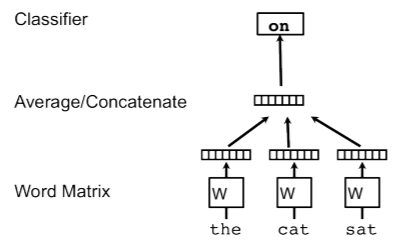
\includegraphics[width=.9\linewidth]{dm}
  \caption{distributed memory}
  \label{fig:dm}
\end{subfigure}%
\begin{subfigure}{.5\textwidth}
  \centering
  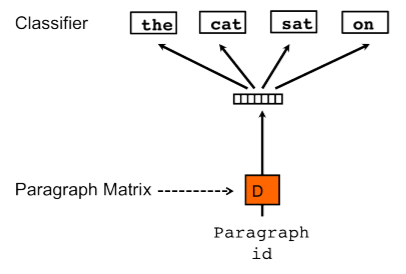
\includegraphics[width=.9\linewidth]{DBOW}
  \caption{distributed bag of words}
  \label{fig:dbow}
\end{subfigure}
\caption{Paragraph vector}
\label{fig:PVDM}
\end{figure}

\begin{figure}[h]
    \centering
	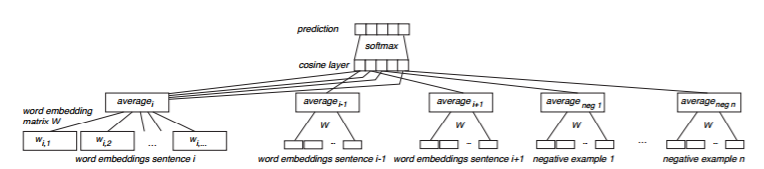
\includegraphics[width=.9\linewidth]{siamesecbow}
    \caption{The architecture of Siamese-CBOW}
    \label{fig:siamese}
\end{figure}
